\documentclass[10pt,twocolumn]{article}
\usepackage[a4paper,margin=18mm,columnsep=7mm]{geometry}
\usepackage[T1]{fontenc}
\usepackage[utf8]{inputenc}
\usepackage{lmodern,microtype,amsmath,amssymb,booktabs,array,graphicx}
\usepackage{algorithm,algpseudocode}
\usepackage[numbers,sort&compress]{natbib}
\usepackage{xcolor,xurl}
\usepackage[hidelinks]{hyperref}
\setlength{\emergencystretch}{2em}
\newcommand{\pending}{\textit{pending}}
% This file contains no transcribed experimental measurements. The generator
% owns every numerical result and protocol value used through these macros.
\InputIfFileExists{generated/macros.tex}{}{}
\InputIfFileExists{generated/forgetting_macros.tex}{}{}
\providecommand{\EvidenceCutoff}{pending evidence cutoff}
\providecommand{\NumCompletedNew}{\pending}
\providecommand{\PrimaryAlpha}{\pending}
\providecommand{\GateBenignRows}{\pending}
\providecommand{\BatchSize}{\pending}
\providecommand{\EpochBudget}{\pending}
\providecommand{\MinSteps}{\pending}
\providecommand{\HiddenWidth}{\pending}
\providecommand{\LearningRate}{\pending}
\providecommand{\MemoryPerClass}{\pending}
\providecommand{\SeedCount}{\pending}
\providecommand{\NSLAACILFPR}{\pending}
\providecommand{\NSLAACILADR}{\pending}
\providecommand{\NSLAACILMFOne}{\pending}
\providecommand{\UNSWAACILFPR}{\pending}
\providecommand{\UNSWAACILADR}{\pending}
\providecommand{\UNSWAACILMFOne}{\pending}
\providecommand{\UNSWExternalADRDelta}{\pending}
\providecommand{\UNSWRegisteredADRDelta}{\pending}
\providecommand{\UNSWRegisteredP}{\pending}
\providecommand{\UNSWTSADR}{\pending}
\providecommand{\UNSWNoAttADR}{\pending}
\providecommand{\NSLFreqADR}{\pending}
\providecommand{\NSLWACBMFOne}{\pending}
\providecommand{\NSLAAFreqADRDelta}{\pending}
\providecommand{\NSLAAFreqP}{\pending}
\providecommand{\UNSWAAExternalP}{\pending}
\providecommand{\NSLAABSDiff}{\pending}
\providecommand{\NSLAABSP}{\pending}
\providecommand{\UNSWAABSDiff}{\pending}
\providecommand{\UNSWAABSP}{\pending}
\providecommand{\UNSWWormsPrecision}{\pending}
\providecommand{\UNSWWormsRecall}{\pending}
\providecommand{\UNSWFuzzersRecall}{\pending}
\providecommand{\BiasClosureUNSW}{\pending}
\providecommand{\BiasClosureCIC}{\pending}
\providecommand{\CICResultStatus}{CIC-IDS-2017 results are incomplete at this snapshot}
\providecommand{\CICPrimaryResultsText}{CIC-IDS-2017 remains a separate generalization test. Until the relevant groups contain all registered seeds, its available rows are descriptive only; no complete-group superiority or safety conclusion is imputed.}
\providecommand{\CICInterpretationText}{The CIC-IDS-2017 comparisons will distinguish the registered restricted-refresh and attack-memory contrasts from the post-hoc Replay-BS contrast when their paired groups are complete. Missing pairs do not establish an architectural or memory benefit.}
\providecommand{\CICConclusionText}{CIC-IDS-2017 contributes only the evidence completed by the stated cutoff; incomplete groups do not extend the present cross-dataset claim.}
\providecommand{\RetentionSelectionText}{The validation-only retention selection remains incomplete.}
\providecommand{\RetentionFormalResultsText}{Complete formal retention groups are not yet available in this snapshot.}
\providecommand{\RetentionDecisionText}{Section 29.8 remains pending; no success is inferred.}
\providecommand{\RetentionComparisonAppendix}{}
\newcommand{\generatedtable}[2]{\InputIfFileExists{generated/#1.tex}{}{\par\noindent\textit{#2: pending generated evidence; no value imputed.}\par}}
\newcommand{\curvefigure}[2]{%
\begin{figure*}[t]\centering
\IfFileExists{figures/#1_operating_curves.pdf}{\includegraphics[width=\textwidth]{figures/#1_operating_curves.pdf}}{\fbox{\parbox[c][23mm][c]{.9\textwidth}{\centering #2 curve pending}}}
\caption{#2 operating curves (post hoc). Threshold-sweep summaries are descriptive, not calibration-set operating points or the registered test. Missing methods or seeds are identified in the generated panel.}\label{fig:curve-#1}\end{figure*}}
\title{Detection and Forgetting under Asymmetric Data Availability in Class-Incremental Network Intrusion Detection}
\author{Wu Liqiang}
\date{Research manuscript --- evidence cutoff: \EvidenceCutoff}
\begin{document}
\raggedbottom
\maketitle
\begin{abstract}
Class-incremental network intrusion detection must retain old attacks while adapting to new traffic. We study whether benign data remaining available outside attack replay memory improve detection without compromising retention. AA-CIL combines a refreshed, independently calibrated benign--attack gate with an attack-only family classifier. At a stagewise benign-calibration target of \PrimaryAlpha\%, its UNSW-NB15 mean incremental balanced accuracy is \UNSWAAIncBAcc\%, final balanced accuracy is \UNSWAAFinalBAcc\%, and forgetting is \UNSWAAForget$\pm$\UNSWAAForgetSD\ percentage points. NSL-KDD forgetting is \NSLAAForget$\pm$\NSLAAForgetSD\ points. Thus favorable detection does not establish successful class retention. UNSW-NB15 attack detection reaches \UNSWAACILADR\%, but its advantage over the strongest registered comparator is only \UNSWRegisteredADRDelta\ points ($p=\UNSWRegisteredP$), failing the original superiority criterion. NSL-KDD test FPR is \NSLAACILFPR\%, demonstrating calibration shift. A post-hoc exposure-matched control supports a dataset-dependent detection benefit, with unmatched total computation. A subsequent validation-only experiment compares five family-retention alternatives under gate distillation; its main version must meet explicit forgetting, final-accuracy and detection requirements before a method-benefit claim is allowed. We preserve negative and incomplete evidence and do not infer novelty or universal superiority. \CICResultStatus.
\end{abstract}
\noindent\textbf{Keywords:} continual learning; intrusion detection; benign data availability; false-positive calibration; replay memory.

\section{Introduction}
Intrusion detection models must recognize newly observed attack families without discarding knowledge of older ones. In class-incremental learning, historical attack records are represented by a limited replay memory, and inference must choose among all observed classes without a task identifier. This constraint is operationally meaningful when previous attack captures cannot be retained indefinitely or reacquired. It does not necessarily imply that benign traffic has the same availability: a monitored network may continue to provide benign examples.

The asymmetry is useful only under an explicit assumption. The learner must have access to a sufficiently clean, representative benign source, distinct from its test data. This paper does not assume that arbitrary production traffic is correctly labeled benign. Nor do we assume that a training-domain benign holdout guarantees the same false-positive rate (FPR) after a distribution change. Both qualifications matter in our results.

Replay-based NIDS research includes class balancing, frequency-aware replacement, representative selection, and other memory designs \citep{cbrs,ecbrs,ssf,acil}. Some multiclass formulations place Normal and attack classes in a common classifier and replay budget. However, this is not a universal description of the literature: binary and novelty-detection methods use different protocols, and prior domain-adaptation work has already used new benign data outside an old attack memory \citep{cerasuolo_rtsi}. The question is therefore not whether benign data have ever been treated differently. It is whether a continuously refreshed, independently calibrated detector provides useful retention and detection behavior in a multistage class-incremental experiment.

We study availability-asymmetric class-incremental learning (AA-CIL). A binary gate $G$ is updated using newly sampled benign data, current attacks, and stored old attacks. A separate classifier $F$ predicts attack families. A benign-only calibration pool sets $G$'s operating threshold without test labels. Memory allocation to attack families is evaluated as a secondary component rather than presented as the principal mechanism.

The contribution is an evidence-bounded experimental study:
\begin{itemize}
\item An explicit separation of persistent attack replay, refreshed benign training data, and permanent benign calibration data, with each storage and training cost disclosed.
\item A modular gate/family design and matched-protocol comparisons that distinguish restricted benign refresh from attack-memory reallocation.
\item A low-false-alarm evaluation reporting actual test FPR, binary attack detection, family-level performance, and negative registered outcomes rather than relying on aggregate accuracy alone.
\item A separately identified post-hoc control, Replay-BS, demonstrating a dataset-dependent difference under matched benign exposure while retaining the limitation of unmatched total computation.
\end{itemize}
These are study contributions, not a declaration that the architecture or its components are individually novel. In particular, the registered strongest-comparator test includes the ablations, and its failure is retained throughout this paper.

\section{Related Work}
\subsection{Replay and class-incremental bias}
iCaRL combines exemplar retention with incremental representation learning \citep{icarl}. Dark Experience Replay and DER++ preserve historical responses alongside supervised rehearsal \citep{der}. These approaches motivate strong replay references, but results obtained with image architectures and original buffering schemes are not automatically reproduced by a tabular NIDS adaptation.

Several methods address old/new-class imbalance. BiC learns a post-training correction \citep{bic}; weight alignment adjusts classifier scale \citep{wa}; separated softmax and taskwise distillation reduce cross-task interference \citep{ssil}; end-to-end incremental learning includes balanced fine-tuning \citep{eeil}. Logit adjustment uses class-prior information to change decision scores \citep{menon}. We use these methods to contextualize earlier diagnostic experiments, not as evidence that a binary gate is a new idea. Adaptation details and their unsuccessful results are retained rather than generalized to the original algorithms.

\subsection{Continual intrusion detection}
CBRS-NIDS distinguishes within-attack and across-class balancing \citep{cbrs}. ECBRS uses frequency-driven replacement and minority protection, while PAPA addresses replay interference \citep{ecbrs}. SSF selects and forgets examples according to their distributional relevance \citep{ssf}. These are predefined \emph{rules}, not necessarily numerically fixed class quotas. SPIDER combines semi-supervised learning and gradient-projection memory, retaining previous-task unlabeled information rather than implementing an all-history equal-class labeled buffer \citep{spider}. CND-IDS studies continual novelty detection with latent regularization and a benign reference set \citep{cndids}. ACIL evaluates multiple memory strategies and reports class-level behavior \citep{acil}. Binary domain-incremental, novelty-detection, and multiclass class-incremental results must not be treated as interchangeable benchmarks.

Our targeted source review found that most of the inspected primary result tables did not separately report benign FPR at a specified operating point. ACIL provides partial or indirect benign-class reporting. This observation motivates explicit operating-point reporting here; it is not a field-wide prevalence estimate or a claim that prior work ignores false alarms.

\subsection{The nearest availability and multistage precedents}
Cerasuolo et al.'s attack-adaptive NIDS uses a multiclass incremental model with exemplars from old benign and attack classes \citep{cerasuolo_comnet}. Their adaptable and explainable NIDS also considers new-domain benign data; it is therefore incorrect to describe its benign information as restricted exclusively to old memory \citep{cerasuolo_eaai}.

The closest availability precedent is their network-agnostic study \citep{cerasuolo_rtsi}. Its adaptation experiment supplies new benign data outside an old memory containing only attacks. This defeats a broad claim that external benign data combined with attack-only old memory is unprecedented. In the inspected experiment, binary detection is derived from multiclass attack outputs, and the evaluation does not establish an independently trained gate that is repeatedly refreshed and FPR-calibrated across multiple attack increments. AA-CIL examines this narrower combination. The absence of an identical verified implementation is not proof of novelty, and a useful incremental contribution must still be isolated experimentally.

Wang and Cao's GLOBECOM paper describes a two-stage class-incremental approach \citep{wangcao}. Only its official abstract and publication record were available for this study. Its stages concern anti-forgetting learning and unbiased prediction; we cannot infer a binary-gate/family architecture, benign refresh policy, or replay exclusion rule from its title. The unavailable full text remains an explicit literature limitation. Finally, TS-mem below is our controlled restricted-refresh ablation, \emph{not} a faithful reproduction of any of these papers.

\section{Problem Analysis}
\subsection{A corrected experimental basis}
The motivating experiments use a taskwise minimum-update schedule rather than only a small fixed number of epochs. This prevents late, rare attack tasks from receiving arbitrarily few optimizer updates. Old attack classes are accessible only through stored training and validation rows after their introduction. Frozen preparation and duplicate/conflict handling are retained across methods; ``deduplicated UNSW-NB15'' does not imply that every benchmark is free of feature collisions or label conflicts. Historical experiments that revisited complete old attack pools are not used as evidence for the present access-constrained protocol. That old-pool resampling was a bug in this project's earlier implementation. The undertraining and data-quality issues identified in that development history are not attributed to published methods without source-specific evidence.

\subsection{False alarms are important, but not a universal root cause}
An earlier decomposition of the historical S2000 DER++ final confusion matrices showed substantial Normal-origin false positives in CIC-IDS-2017 attack-family columns, including families with high recall but low precision. These DER++ proportions must not be assigned to every method. UNSW-NB15 also exhibited attack-to-attack confusions and lost attack recall. These observations justify measuring benign FPR and attack detection separately, but do not identify inadequate benign coverage or Normal--attack memory competition as a universal causal explanation. The decomposition is arithmetic, not an intervention proving a mechanism.

Under the registered correction sweep, the best tested correction/base combinations closed only \BiasClosureUNSW\% and \BiasClosureCIC\% of the positive Joint-minus-incremental Macro-F1 gaps on UNSW-NB15 and CIC-IDS-2017, respectively. This rejects the sufficiency of those specific adaptations and candidate ranges, not bias correction in general. Joint is an offline reference rather than a guaranteed numerical upper bound.

\subsection{Why change the learning organization?}
The preceding FARQ experiments adjusted shared replay allocation using measured validation false alarms. Their registered main criterion failed, and descriptive operating curves did not establish a universally superior false-alarm/detection frontier. Replay+LA and Replay share the same attainable predictions when the total adjustment is recalibrated; this does not make all allocation methods threshold-equivalent. WACB and Freq change the learned model and improve detection relative to Replay at evaluated matched-FPR points on UNSW-NB15 and CIC-IDS-2017. Memory reallocation can therefore improve the measured trade-off, although it does not close every offline-reference gap. These finite operating-point comparisons are not a global frontier theorem. AA-CIL tests a different learning organization, not a premise that every shared-classifier method merely moves along one common curve.

\section{Method: AA-CIL}
\subsection{Data roles and access assumption}
At update $t$, let $\mathcal A_t$ be the observed attack families and $\mathcal N_t$ the newly introduced attack families. The learner receives their current training data $D_t^A$, retained old attack training memory $R_{t-1}^{A,\mathrm{tr}}$, and a benign training source $B^{\mathrm{tr}}$. A permanent benign calibration pool $B^{\mathrm{cal}}$ is disjoint from every optimizer input. We assume continued access to $B^{\mathrm{tr}}$ but not to the original pools of old attacks.

The benchmark simulates benign availability by drawing a task-dependent sample $B_t\subseteq B^{\mathrm{tr}}$ of up to \GateBenignRows\ rows. Samples may overlap across tasks; this is repeated access to a fixed prepared training source, not evidence from a newly collected live stream. The permanent split prevents a calibration row from later becoming a training row.

\subsection{Independent detector and family learner}
The gate is a binary MLP trained on
\begin{equation}
 D_t^G=B_t\cup D_t^A\cup R_{t-1}^{A,\mathrm{tr}}.
\end{equation}
Its labels are benign versus attack. The family MLP is trained on
\begin{equation}
 D_t^F=D_t^A\cup R_{t-1}^{A,\mathrm{tr}},
\end{equation}
using attack-family labels only. Both use the existing class-balanced cross-entropy implementation and retain learned parameters between updates. Their optimizers and costs are separate. Neither model receives calibration data as optimization input.

For exact implementation fidelity, the family network is initialized with the benchmark's full attack-label output dimension. Training follows the shared replay cross-entropy implementation, while inference restricts the argmax to observed attack families. Thus this experiment assumes a known finite benchmark label universe; it is not a claim about an unbounded, dynamically expanding unknown-label vocabulary.

\begin{figure*}[t]
\centering
\IfFileExists{figures/architecture.pdf}{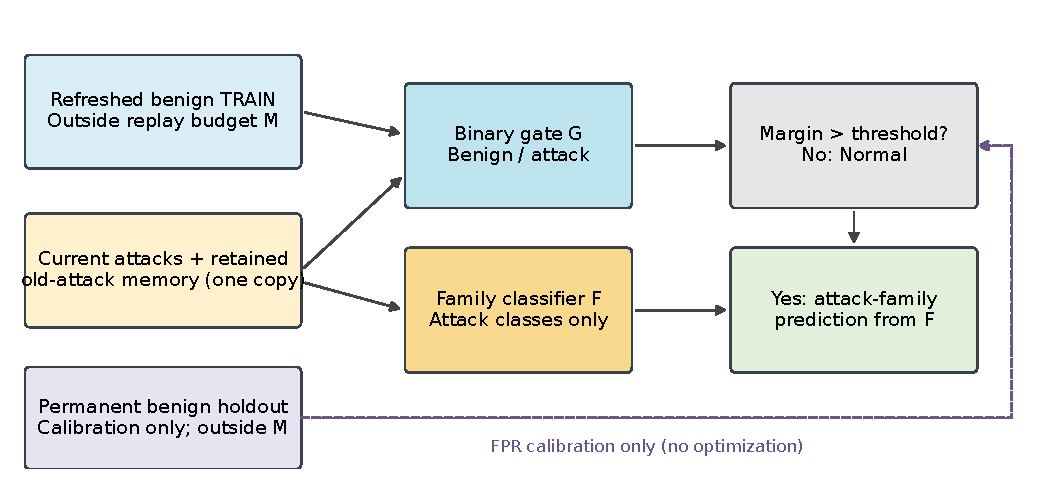
\includegraphics[width=\textwidth]{figures/architecture.pdf}}{\fbox{\parbox[c][30mm][c]{.9\textwidth}{\centering Architecture diagram pending vector rendering}}}
\caption{AA-CIL separates detection from family classification. The calibration pool never enters training. A single retained attack memory supplies both learners and is counted once; two networks and both training schedules are counted in cost.}
\label{fig:architecture}
\end{figure*}

\subsection{Attack replay allocation}
Let $K_t=|\mathcal A_t|+1$, including Normal, and let $m$ be the common per-observed-class budget. The shared capacity is
\begin{equation}
 M_t=mK_t,\qquad m=\MemoryPerClass.
\end{equation}
AA-CIL divides $M_t$ among observed attacks: $q_{t,c}=\lfloor M_t/|\mathcal A_t|\rfloor$ plus one for the first remainder classes in ascending class-ID order. This is a capacity ceiling, not a promise of equal actual occupancy. Each class allocation contains separate training and validation slots; validation rows do not enter optimization. When a class is new, examples can be selected from its prepared training and validation partitions. Once it is old, the corresponding retained arrays are the only permissible source, even if a later quota exceeds available rows. Unused slots remain unused; old pools are never revisited to fill them.

This allocation transfers the nominal Normal share to attacks. It does not make benign data free in a physical-storage sense: both benign training samples and the permanent calibration pool are disclosed outside $M_t$. The no-transfer ablation tests whether this allocation adds value beyond benign refresh.

\subsection{Calibration and inference}
Let $s_G(x)=z_A(x)-z_B(x)$ be the gate's attack-minus-benign logit margin. For $n=|B^{\mathrm{cal}}|$, sort its margins as $s_{(1)}\leq\cdots\leq s_{(n)}$ and set
\begin{equation}
 k_\alpha=\lfloor\alpha n\rfloor,\qquad
 q_{t,\alpha}=s_{(n-k_\alpha)}.
\end{equation}
The strict decision $s_G(x)>q_{t,\alpha}$ bounds the empirical calibration false-alarm count by $k_\alpha$, including ties. No randomized tie breaking is used. Prediction is
\begin{equation}
 \hat y(x)=\begin{cases}
 \mathrm{Normal},&s_G(x)\leq q_{t,\alpha},\\
 \arg\max_{c\in\mathcal A_t}F_c(x),&s_G(x)>q_{t,\alpha}.
 \end{cases}
\end{equation}
This is an empirical training-holdout operating point, not a distribution-free guarantee on test or deployment FPR. Gate false negatives cannot be recovered by the downstream family classifier.

\begin{algorithm}[t]
\caption{One AA-CIL update}
\label{alg:aacil}
\begin{algorithmic}[1]
\Require Current attacks $D_t^A$; retained attack memory $R_{t-1}^A$; benign pools $B^{\mathrm{tr}},B^{\mathrm{cal}}$
\State Sample $B_t$ from $B^{\mathrm{tr}}$ only.
\State Train $G$ on $B_t\cup D_t^A\cup R_{t-1}^{A,\mathrm{tr}}$.
\State Train $F$ on $D_t^A\cup R_{t-1}^{A,\mathrm{tr}}$.
\State Allocate attack capacities $q_{t,c}$ within $M_t$.
\For{each observed attack $c$}
\State Select new-class rows, or subsample retained old rows; keep training and validation disjoint.
\EndFor
\State Calibrate $q_{t,\alpha}$ on $B^{\mathrm{cal}}$; do not update weights.
\State Save models, retained memory, allocation, costs, and operating-point confusion matrices.
\end{algorithmic}
\end{algorithm}

\subsection{Post-hoc retention extension: AA-CIL-KD}
The original AA-CIL gate relies on attack replay without an explicit response-retention loss, and its family learner uses ordinary replay. AA-CIL-KD is a post-hoc extension to that study, with its protocol and success criteria registered before observing any KD results. It adds a gate loss
\begin{equation}
 \mathcal L_G=\mathcal L_{\mathrm{CE},G}
       +\lambda_G\,\mathcal L_{\mathrm{MSE},G}.
\end{equation}
For retained old attack training rows, the gate targets are the stored two-logit responses recorded when those rows entered memory. For the current benign sample, targets come from the frozen preceding-task gate. New attack rows have no old-class distillation target, and the first task has no preceding-task gate. Neither calibration rows nor attack validation rows become optimizer inputs.

The attack-only family learner uses a task-boundary DER++-objective adaptation: supervised learning is supplemented by replay cross-entropy and MSE against stored family logits. This is not a claim to reproduce the original DER++ online storage schedule. Gate and family logits are auxiliary records for the same attack rows, not two separately allocated sample memories; their storage and the two training costs must be disclosed. The update budgets, benign refresh, permanent holdout and threshold policy remain those of AA-CIL.

An initial development search used mean stagewise validation balanced accuracy and varied three distillation coefficients. It was superseded before formal KD results by the retention-constrained selection below. Its completed runs remain part of the development cost, but do not enter the new selection. The previously planned noGKD ablation is not one of the five family-model candidates in this revised experiment.

\subsection{Post-hoc parameter isolation: AA-CIL-ISO}
AA-CIL-ISO changes only the family learner relative to AA-CIL-KD: the gate, G-KD objective, benign refresh and calibration remain the same. It uses the existing MLP feature encoder, not a transplanted transformer pipeline. On the first task containing attacks, the encoder and that task's new family heads train jointly within one family-model update budget. The encoder is then frozen. Each new family $c$ receives its own rank-8 residual adapter and two-logit binary head,
\begin{equation}
 h_c=h+U_cV_ch,\qquad p_c(x)=\operatorname{softmax}(H_ch_c)_1.
\end{equation}
The head learns that family versus the other attacks available in the current task and legal old-attack replay. Multiple new families provide negatives for one another. Normal rows are not used as family-head negatives. After the task, its adapters and heads are frozen permanently; old attack pools are never reopened.

All heads introduced in one task share a single training loop: their class-balanced binary cross-entropies are averaged before each optimizer step. Each new head participates in the task's common $\max(8\text{ epochs},2000\text{ steps})$ schedule, rather than receiving an additional serial budget per head. The first encoder training has no separate pretraining budget. Joint family-loop time and shared steps are recorded once; exclusive per-head time is not inferred from that total. If the first task contains only one attack family, there are no other-attack negatives: this limitation is recorded explicitly, without invented negatives or benign substitution.

After the gate declares an attack, prediction is $\arg\max_{c\in\mathcal A_t}p_c(x)$ over independently normalized positive probabilities. This is head-only inference with no router and no cross-head softmax calibration. It adapts OFRA-style parameter isolation to the present backbone and protocol; historical OFRA forgetting values do not establish its performance here. ISO is evaluated under the newly registered retention and detection criteria, with descriptive paired comparisons against KD. No ISO success is inferred before those results are available.

\subsection{Retention alternatives and validation-only selection}
The revised experiment compares five family learners under the same G-KD gate: KD, ISO, weight alignment (WA), class-balanced fine-tuning (CBF), and nearest-class-mean prediction (NCM). WA rescales newly introduced classifier weights by the mean old-to-new weight-norm ratio after task training \citep{wa}. CBF adds small-learning-rate updates on balanced retained attack training memory \citep{eeil}. NCM computes class prototypes from retained attack training rows encoded by the current family encoder and predicts by feature-space distance \citep{icarl}. These are adaptations of established mechanisms, not claims of novel versions of the cited algorithms. Their additional time, steps, prototype storage and model storage are reported separately.

Only UNSW-NB15 development seeds $\{5,6\}$ select hyperparameters and the main version. Each candidate uses $\lambda_G\in\{0.5,1,2\}$; KD fixes both family DER coefficients to one. CBF uses $0.1$ times the base learning rate and either one or five fine-tuning epochs. A stratified permanent $10\%$ attack holdout supplies fixed validation cohorts across stages; it is never optimized, is accessible only for this development evaluation, and its storage is disclosed outside the replay budget. The permanent Normal holdout supplies the gate threshold at $\alpha=2\%$ and the Normal validation cohort. This development-only access exception does not reopen old attack training pools or change formal replay access.

For each version, eligible configurations have final validation balanced accuracy at least the original AA-CIL development mean minus three percentage points. The configuration with lowest mean validation forgetting is retained, and the lowest-forgetting eligible version is selected as the candidate main method. All choices are frozen across datasets before evaluation seeds $\{1,2,3,4,42\}$ are used. Every version is reported, not only the selected one. If no configuration is eligible, there is no eligible main method; any configuration retained for descriptive formal reporting is explicitly a fallback, not an eligibility success. Test labels never select the gate threshold, hyperparameters, or main version.

\section{Experimental Setup}
\subsection{Benchmarks and task protocol}
We use the prepared NSL-KDD, deduplicated UNSW-NB15, and CIC-IDS-2017 benchmarks \citep{nsl,unsw,cic}. Normal and an initial attack family appear in the first task, followed by the fixed attack-family sequence. The data manifest and generated protocol table specify label mappings, task groupings, split sizes, and feature dimensions. Test rows from unobserved classes are excluded at intermediate checkpoints; final metrics use the complete prepared test set. No test row is selected for training, memory construction, or primary calibration.
\generatedtable{protocol}{Dataset and protocol table}
\generatedtable{dataset_details}{Dataset preparation and task details}

Training uses MLPs with two hidden layers of width \HiddenWidth, Adam with learning rate \LearningRate, and batch size \BatchSize. Each model/update receives
\begin{equation}
 S_t=\max\!\left(\MinSteps,\EpochBudget\left\lceil |D_t|/\BatchSize\right\rceil\right)
\end{equation}
optimizer steps. Consequently, matching this schedule does not imply identical realized steps when data exposure differs. Gate and family schedules are recorded separately. The registered seed set contains \SeedCount\ seeds; tables report actual completed $n$ where the cutoff prevents a complete group. Partial groups are not silently replaced with selected favorable seeds.

The observed local GPU is an NVIDIA GeForce RTX 4060 Ti with 8 GiB memory; the HPC execution environment uses NVIDIA A100 GPUs. HPC results are included only after completed execution, not merely submission or allocation. Heterogeneous hardware and shared local GPU use mean that reported runtimes are not a controlled hardware benchmark.

\subsection{Comparators and ablations}
The external comparison set is Replay, DER++, WACB, Freq, and Replay+LA. Replay uses the common tabular architecture. DER++ is the recorded tabular adaptation with classwise memory management, not an exact replication of the original vision protocol. WACB adapts benign-versus-combined-attack balancing to this multiclass setting. Freq is a simplified frequency-proportional allocation control, not an exact ECBRS reproduction. Replay+LA is a saved-model logit-adjustment evaluation; it is not an additional independently trained network. All primary operating thresholds are determined from the same permanent benign calibration pool.

TS-mem retains the same gate/family organization but restricts each task's benign refresh to the training portion of the ordinary Normal allocation, while sharing replay capacity between Normal and attacks. It therefore measures a restricted benign exposure policy, not the effect of a frozen benign subset alone. AA-noAttMem retains refreshed benign training and the independent gate but does not transfer the Normal allocation to attacks. Its name does not mean that attacks have no replay memory.

Joint trains with the offline data available under its recorded protocol and is reported as a reference. It is not a guaranteed upper bound, a matched-storage online learner, or a member of the strongest-baseline selection. FARQ is supplementary. The registered selection includes the external methods \emph{and} TS-mem and AA-noAttMem; excluding those ablations after inspecting results would change the registered question.

\subsection{Metrics and registered inference}
For confusion counts $C_{ij}$ with Normal index $b$, we report
\begin{align}
 \mathrm{FPR}&=\frac{\sum_{j\ne b}C_{bj}}{\sum_j C_{bj}},\\
 \mathrm{ADR}&=\frac{\sum_{i\ne b}\sum_{j\ne b}C_{ij}}{\sum_{i\ne b}\sum_j C_{ij}}.
\end{align}
ADR is binary attack detection, not correct-family recall. Macro-F1 and attack-family macro recall supplement it. The registered family-recall guard includes attack classes meeting the specified minimum test support; excluded rare classes remain visible in per-class evidence. Precision is undefined for a class with no predictions in a seed and is never changed to zero. Its group mean and sample standard deviation use only defined seed values, with the actual $n_{\mathrm{defined}}$ (\texttt{defined\_n}) reported separately from the total seed count. If none are defined, the mean remains undefined; with fewer than two defined values, the sample standard deviation is undefined. Such a seed is not dropped from recall, forgetting, or other defined endpoints.

The primary calibration target is $\alpha=\PrimaryAlpha\%$. Actual test FPR is reported alongside it because equal calibration targets need not yield equal test FPR. The primary registered superiority criterion requires a one-sided paired test against the highest-mean registered comparator in at least two datasets. The comparator is chosen once per dataset and endpoint from whole-seed means, not separately per seed. Other criteria test Macro-F1 harm, the family-recall guard, the CIC gate-refresh ablation, and descriptive cost/Joint reporting. Paired differences, sample standard deviations, and effect sizes accompany tests where available. No multiplicity correction was registered; selection of the highest observed mean and the small seed count limit inferential strength. A nonsignificant difference is not an equivalence or noninferiority result.

\section{Results}
\subsection{Class-incremental retention and forgetting}
Class-incremental performance is evaluated before the false-alarm--detection comparison. For every saved checkpoint $t=1,\ldots,T$, the operating threshold is determined anew from the same permanent Normal calibration pool at $\alpha=2\%$, using that checkpoint's scores. The final threshold is not retrospectively applied to earlier models. For a seen class $c$, let $r_{c,t}$ denote its recall under this operating point and let $\mathcal C_t$ be the seen-class set. We report
\begin{align}
 B_t&=\frac{1}{|\mathcal C_t|}\sum_{c\in\mathcal C_t}r_{c,t}, &
 \overline B_{\mathrm{inc}}&=\frac{1}{T}\sum_{t=1}^{T}B_t,
\end{align}
together with final balanced accuracy $B_T$. Mean incremental balanced accuracy weights stages equally, rather than pooling their examples or reporting micro accuracy.

Let $\tau_c$ be the introduction stage of class $c$ and $\mathcal O=\{c:\tau_c<T\}$. Signed final forgetting is
\begin{equation}
 \mathcal F=\frac{1}{|\mathcal O|}\sum_{c\in\mathcal O}
 \left(\max_{\tau_c\leq t<T}r_{c,t}-r_{c,T}\right).
\end{equation}
The historical maximum excludes the final stage; negative values therefore retain final improvement and are not clipped to zero. The primary definition includes Normal whenever it belongs to $\mathcal O$; an attack-only version excludes Normal from this same set. Classes introduced in the final task have no subsequent update and are not assigned a forgetting value. No rare-class support filter is applied to these Class-IL summaries: the support filter belongs only to the separate attack-family safety guard. We report per-seed values and their mean and sample standard deviation, with forgetting in percentage points. Low forgetting alone is not a ranking of useful retention: a class that was never learned well has little recall to lose. It must be read together with final and mean incremental balanced accuracy for every method. Incomplete trajectories or seed groups remain explicitly incomplete.
\generatedtable{forgetting_results}{Checkpoint-calibrated Class-IL results}

The completed original-AA trajectories show why detection and retention must be separated. On UNSW-NB15, mean incremental BAcc is \UNSWAAIncBAcc\%, final BAcc is \UNSWAAFinalBAcc\%, and signed forgetting is \UNSWAAForget$\pm$\UNSWAAForgetSD\ percentage points. On NSL-KDD, the corresponding values are \NSLAAIncBAcc\%, \NSLAAFinalBAcc\%, and \NSLAAForget$\pm$\NSLAAForgetSD\ points. A higher trajectory average therefore coexists with substantial old-class recall loss; the new KD and ISO variants target that unresolved endpoint rather than converting the earlier detection gain into a retention claim.

For each old attack class, the confusion matrix partitions its error into a gate miss (prediction Normal) and a wrong attack-family prediction. At the same class-specific pre-final peak used above, the recall loss equals the increase in these two error rates. The decomposition uses their common class support and common peak checkpoint; it does not sum independently selected worst stages. It separates observed routing errors, not a causal proof that weight interference alone caused forgetting, because every checkpoint also receives its own calibrated threshold.
\generatedtable{forgetting_decomposition}{Gate and family components of forgetting}

The revised pre-formal decision rule (Section 29.8 of the work order, superseding Section 29.4) makes retention mandatory. On both UNSW-NB15 and NSL-KDD, the validation-selected version must have no significantly greater forgetting than the lowest-forgetting external baseline, significantly higher final balanced accuracy than exposure-matched Replay-BS, and no significantly lower $\alpha=2\%$ attack detection than original AA-CIL. The external set is Replay, DER++, WACB, Freq and Replay+LA; one comparator is chosen from each complete five-seed group mean, never per seed. Tests are paired, one-sided, at $p<0.05$. CIC-IDS-2017 is reported as available and does not replace either required dataset. Mean incremental balanced accuracy, Macro-F1 and FPR remain mandatory descriptive outcomes. Failure of any necessary condition leaves the false-alarm--forgetting trade-off unresolved and precludes a successful method-contribution claim. Incomplete groups remain incomplete. This revised experiment cannot overwrite the failed original Section 27.8 test, and nonsignificant harm is not proof of equivalence or noninferiority.

\RetentionSelectionText
\generatedtable{retention_selection}{Locked validation-only retention selection}
\RetentionFormalResultsText
\generatedtable{retention_results}{Formal five-version retention results}
\RetentionDecisionText
The supplemental Section 29.8 CIC-IDS-2017 job reached the scheduler's \texttt{DEADLINE} state without an allocation or any execution, yielding no scientific results; this is missing evidence, not a negative model outcome.

\subsection{Primary calibration-set operating points}
Table~\ref{tab:main-results} reports all available methods at the common calibration target, including actual test FPR and completed seed counts. \CICResultStatus. The cutoff is \EvidenceCutoff; an unavailable cell denotes unfinished evidence, not zero performance.
\IfFileExists{generated/main_results.tex}{%
\AddToHookNext{env/table*/end}{\par\vspace{2pt}\begin{minipage}{.98\linewidth}\footnotesize
Exposure confound: AA-CIL and AA-noAttMem refresh up to 50,000 benign training rows per task outside replay memory. After Normal's introduction, ordinary replay controls use quota-limited Normal training memory. Their ADR differences therefore cannot be attributed wholly to the gate/family structure. Post-hoc Replay-BS matches the added benign exposure and attack allocation, but not the two-model total computation.
\end{minipage}}%
\begin{table*}[t]
\centering\scriptsize
\setlength{\tabcolsep}{3.8pt}
\caption{Final-task test performance at a benign-holdout calibration target of $\alpha=2\%$. Rates are percentages; mean $\pm$ sample SD. Actual test FPR is not fixed at 2\%.}\label{tab:main-results}
\begin{tabular}{llrrrrrr}
\toprule
Data & Method & n & Test FPR & Attack detection & Macro-F1 & BAcc & Attack guard \\
\midrule
NSL & Replay & 5 & 4.08$\pm$2.16 & 65.39$\pm$5.30 & 46.83$\pm$4.93 & 47.05$\pm$4.52 & 34.83$\pm$5.78 \\
NSL & DER++ & 5 & 2.51$\pm$0.45 & 65.28$\pm$2.73 & 50.46$\pm$3.15 & 50.11$\pm$2.97 & 38.27$\pm$3.77 \\
NSL & WACB & 5 & 3.62$\pm$0.87 & 66.83$\pm$3.77 & 57.03$\pm$3.91 & 56.69$\pm$5.22 & 46.77$\pm$6.49 \\
NSL & Freq & 5 & 4.93$\pm$2.42 & 69.67$\pm$2.53 & 56.84$\pm$4.32 & 61.82$\pm$2.44 & 53.50$\pm$3.50 \\
NSL & Replay+LA & 5 & 4.08$\pm$2.16 & 65.39$\pm$5.30 & 46.83$\pm$4.93 & 47.05$\pm$4.52 & 34.83$\pm$5.78 \\
NSL & TS-mem & 5 & 4.41$\pm$2.12 & 63.19$\pm$4.66 & 51.44$\pm$2.16 & 55.62$\pm$1.58 & 45.62$\pm$1.92 \\
NSL & AA-noAttMem & 5 & 4.32$\pm$1.82 & 60.29$\pm$3.16 & 56.67$\pm$3.34 & 56.97$\pm$2.69 & 47.29$\pm$3.05 \\
NSL & AA-CIL & 5 & 6.15$\pm$1.79 & 62.84$\pm$3.46 & 55.66$\pm$3.36 & 58.26$\pm$1.85 & 49.36$\pm$1.98 \\
NSL & Replay-BS (post hoc) & 5 & 3.65$\pm$2.16 & 62.48$\pm$4.64 & 57.05$\pm$3.33 & 59.32$\pm$2.85 & 50.07$\pm$3.92 \\
NSL & Joint (offline) & 5 & 6.79$\pm$1.00 & 66.63$\pm$1.80 & 59.37$\pm$2.90 & 58.65$\pm$2.20 & 50.01$\pm$2.75 \\
UNSW & Replay & 5 & 1.78$\pm$0.20 & 38.52$\pm$3.77 & 26.27$\pm$0.85 & 25.15$\pm$0.89 & 17.04$\pm$0.98 \\
UNSW & DER++ & 5 & 1.98$\pm$0.27 & 18.48$\pm$4.12 & 14.47$\pm$1.44 & 14.43$\pm$1.03 & 5.15$\pm$1.16 \\
UNSW & WACB & 5 & 1.93$\pm$0.24 & 48.97$\pm$4.14 & 32.81$\pm$1.18 & 29.96$\pm$1.30 & 22.39$\pm$1.46 \\
UNSW & Freq & 5 & 2.01$\pm$0.26 & 50.42$\pm$2.93 & 31.22$\pm$1.73 & 28.93$\pm$1.40 & 21.25$\pm$1.54 \\
UNSW & Replay+LA & 5 & 1.78$\pm$0.20 & 38.52$\pm$3.77 & 26.27$\pm$0.85 & 25.15$\pm$0.89 & 17.04$\pm$0.98 \\
UNSW & TS-mem & 5 & 1.98$\pm$0.12 & 24.79$\pm$14.93 & 23.47$\pm$6.33 & 24.97$\pm$7.34 & 16.85$\pm$8.15 \\
UNSW & AA-noAttMem & 5 & 1.94$\pm$0.19 & 67.94$\pm$1.58 & 40.43$\pm$0.51 & 53.98$\pm$1.02 & 49.09$\pm$1.12 \\
UNSW & AA-CIL & 5 & 1.92$\pm$0.15 & 69.09$\pm$0.93 & 41.18$\pm$0.28 & 55.05$\pm$1.06 & 50.27$\pm$1.18 \\
UNSW & Replay-BS (post hoc) & 5 & 2.13$\pm$0.17 & 66.14$\pm$0.74 & 39.99$\pm$1.57 & 38.01$\pm$1.19 & 31.36$\pm$1.31 \\
UNSW & Joint (offline) & 5 & 1.93$\pm$0.15 & 67.11$\pm$1.45 & 37.22$\pm$1.00 & 35.38$\pm$0.67 & 28.42$\pm$0.76 \\
CIC17 & Replay & 5 & 1.95$\pm$0.06 & 78.89$\pm$5.63 & 51.52$\pm$4.02 & 52.32$\pm$4.55 & 47.87$\pm$6.55 \\
CIC17 & DER++ & 5 & 1.92$\pm$0.07 & 89.29$\pm$3.01 & 48.85$\pm$3.19 & 48.44$\pm$2.90 & 47.68$\pm$3.63 \\
CIC17 & WACB & 5 & 1.92$\pm$0.06 & 88.91$\pm$2.30 & 57.84$\pm$1.13 & 63.02$\pm$1.31 & 59.90$\pm$0.67 \\
CIC17 & Freq & 5 & 1.93$\pm$0.02 & 88.55$\pm$2.32 & 57.97$\pm$4.33 & 64.03$\pm$2.62 & 61.81$\pm$5.97 \\
CIC17 & Replay+LA & 5 & 1.95$\pm$0.06 & 78.89$\pm$5.63 & 51.52$\pm$4.02 & 52.32$\pm$4.55 & 47.87$\pm$6.55 \\
CIC17 & TS-mem & 5 & 1.89$\pm$0.06 & 49.51$\pm$3.90 & 34.63$\pm$2.25 & 40.34$\pm$2.01 & 26.88$\pm$2.99 \\
CIC17 & AA-noAttMem & 5 & 1.94$\pm$0.03 & 83.13$\pm$1.48 & 63.60$\pm$0.78 & 87.50$\pm$0.35 & 89.21$\pm$0.46 \\
CIC17 & AA-CIL & 0 & -- & -- & -- & -- & -- \\
CIC17 & Replay-BS (post hoc) & 4 & 1.94$\pm$0.03 & 92.62$\pm$1.24 & 69.03$\pm$1.05 & 79.39$\pm$4.16 & 82.56$\pm$5.86 \\
CIC17 & Joint (offline) & 5 & 1.93$\pm$0.04 & 98.19$\pm$1.94 & 68.43$\pm$1.30 & 78.68$\pm$3.54 & 78.56$\pm$3.58 \\
\bottomrule
\end{tabular}
\par\vspace{2pt}\begin{minipage}{.98\linewidth}\footnotesize Replay+LA and Replay share the same calibrated total logit adjustment and weights. Joint has offline old-training access. Replay-BS is post hoc. A dash means unavailable; $n<5$ is descriptive only. The guard alone excludes attack classes with test support below 20.\end{minipage}
\end{table*}
%
}{\generatedtable{main_results}{Primary operating-point results}}

On UNSW-NB15, AA-CIL obtains ADR \UNSWAACILADR\%, Macro-F1 \UNSWAACILMFOne\%, and test FPR \UNSWAACILFPR\%. Relative to the strongest \emph{external} ADR baseline, the gain is \UNSWExternalADRDelta\ percentage points. This comparison is descriptive with an associated paired test, distinct from the registered strongest-comparator conclusion.

High binary detection does not imply accurate attack naming: AA-CIL's UNSW-NB15 Worms recall is \UNSWWormsRecall\%, but precision is only \UNSWWormsPrecision\%; Fuzzers recall is \UNSWFuzzersRecall\%. The appendix retains these difficult-family results rather than using ADR to conceal family-level errors.

On NSL-KDD, AA-CIL reaches ADR \NSLAACILADR\%, compared with \NSLFreqADR\% for Freq. Its Macro-F1 is \NSLAACILMFOne\%, compared with \NSLWACBMFOne\% for WACB. Its test FPR, \NSLAACILFPR\%, is substantially different from the calibration target. The method therefore neither wins across benchmarks nor delivers the nominal low-FPR operating point on this shifted test distribution.

\CICPrimaryResultsText

\subsection{The registered conclusion remains negative}
On UNSW-NB15, the strongest registered ADR comparator is AA-noAttMem, not Freq. AA-CIL's paired mean advantage is \UNSWRegisteredADRDelta\ percentage points, with one-sided $p=\UNSWRegisteredP$. It does not pass the registered significance criterion. NSL-KDD also fails the superiority requirement. Even a favorable CIC-IDS-2017 result cannot then provide superiority in the required majority of datasets. The primary registered criterion and conjunction are therefore negative; remaining individual criteria retain their actual complete or incomplete states.
\generatedtable{registered_criteria}{Registered criterion-by-criterion decision}

This result is not revised by restricting the baseline set to external methods. The external comparison answers a useful but different question: whether the complete configuration improves upon the selected standard replay alternatives. Both comparisons are shown, and neither is described as a proof of equivalence.

\subsection{What the ablations identify}
\generatedtable{ablation_results}{Availability and memory ablations}
The UNSW-NB15 contrast between TS-mem (ADR \UNSWTSADR\%) and AA-noAttMem (\UNSWNoAttADR\%) is consistent with a substantial benefit from greater benign refresh within the two-model design. The latter retains ordinary attack allocations, so attack-memory transfer is not required to observe this particular gain. However, the comparison also changes benign sample exposure, realized gate updates, and temporary storage. It does not by itself prove that the architecture, rather than the additional training data, causes the improvement.

The AA-CIL--AA-noAttMem contrast is the evidence for attack-memory transfer. Its UNSW-NB15 detection difference is small relative to the external-baseline gap and is not significant in the registered one-sided test. This makes memory transfer a secondary, presently weakly supported component. It does not establish zero benefit, equivalence, or dispensability on every dataset.

\subsection{Post-hoc exposure-matched and shift analyses}
Replay-BS was requested after the initial results. It supplies a single multiclass replay model with the same refreshed benign samples, attack-only memory capacity, current attacks, and calibration policy as AA-CIL. It is the necessary control for distinguishing decomposition from the broader benign-access setting. Its evidence is reported separately and cannot retroactively rescue the registered criterion.
\generatedtable{replay_bs}{Post-hoc Replay-BS comparison}

The complete NSL-KDD and UNSW-NB15 groups now permit this comparison. On UNSW-NB15, AA-CIL improves attack detection over Replay-BS by \UNSWAABSDiff\ percentage points in the post-hoc paired test ($p=\UNSWAABSP$; Table~\ref{tab:ablation-results}), despite matching the additional benign exposure and replay-allocation rule. This supports an incremental benefit of the decomposed configuration beyond merely providing more benign examples under this protocol. On NSL-KDD, the difference is only \NSLAABSDiff\ points ($p=\NSLAABSP$), and AA-CIL has higher test FPR and lower Macro-F1 than Replay-BS. Hence the evidence is dataset dependent, not a general architectural advantage. Moreover, the two-model system still has a separate family-training budget, so this is not a compute-matched causal isolation of architecture.

The completed NSL sensitivity analysis contrasts thresholds calibrated using training-domain benign holdout data with thresholds estimated from test-domain Normal data. The latter deliberately uses test information and is therefore diagnostic only: it must not replace the primary result, be called a deployment-valid evaluation, or be used to select a favorable main threshold. Test-Normal calibration brings the measured false-alarm rate to the target by construction but reduces attack detection and Macro-F1 for the evaluated gate variants (Table~\ref{tab:calibration-shift}). The original discrepancy is consequently not resolved as a free improvement: threshold tightening exposes a detection cost, while the same-population calibration cannot establish out-of-sample reliability.
\generatedtable{calibration_shift}{Post-hoc calibration-shift sensitivity}

The operating curves in Figs.~\ref{fig:curve-nsl_kdd}--\ref{fig:curve-cic_ids_2017} are also post hoc. A mean curve at a common threshold is not the same estimand as averaging per-seed interpolated detection at a fixed FPR. Finite-grid points without a bracket remain unavailable; they are not extrapolated to make all methods comparable. A visually favorable curve does not replace the calibration-holdout test or its registered inference.
\curvefigure{nsl_kdd}{NSL-KDD}
\curvefigure{unsw_nb15}{UNSW-NB15}
\curvefigure{cic_ids_2017}{CIC-IDS-2017}

\subsection{Cost and storage}
\generatedtable{joint_gaps}{Descriptive gaps from the offline reference}
\generatedtable{costs}{Training and storage costs}
We charge the gate and family model separately and report their sum. Selection, calibration, evaluation, and additional benign sample storage are separate quantities. A common replay capacity does not make AA-CIL compute-matched to a single-network baseline. Nor does a common maximum memory establish equal occupancy: rare old classes may exhaust their retained samples and leave slots unused.

The permanent benign pool and the extra benign training inputs of AA-CIL, AA-noAttMem and Replay-BS are outside the replay ceiling but inside the disclosed total data footprint. TS-mem instead uses its retained Normal training rows within the ceiling. Normal validation rows already counted within TS-mem's replay allocation are not counted again as additional unique calibration rows. Successful optimization time excludes loading and serialization unless explicitly stated. Local GPU sharing and heterogeneous execution devices preclude interpreting raw runtime differences as an exclusive hardware benchmark. Failed, duplicate, or superseded executions are not scientific replicates and are accounted for separately from selected successful-cell costs.

\section{Discussion and Limitations}
\subsection{A useful result without a universal winner}
The strongest supported observation is dataset dependent: independently calibrated benign-refresh models substantially improve the selected external-baseline comparison on UNSW-NB15, whereas NSL-KDD does not improve the relevant registered endpoints. The evidence does not support a blanket superiority claim. In particular, favorable binary ADR can coexist with poor family discrimination: detected attacks assigned to the wrong family count as detected in ADR but not as correct in the multiclass metrics.

The work also separates a design hypothesis from its identification. TS-mem shows the outcome of restricting benign refresh within a two-model architecture. The completed Replay-BS comparison strengthens the UNSW-NB15 evidence beyond an explanation based solely on additional benign exposure. Its NSL-KDD result does not support the same benefit, and its single network still receives less total model training than the gate-plus-family configuration. The supported claim is therefore an exposure-matched, dataset-dependent configuration benefit, not a compute-isolated causal estimate of decomposition.

\CICInterpretationText\ Regardless of this additional comparison, the failed original superiority requirement is unchanged. A CIC-only gain would not establish a universal advantage, and a post-hoc curve or Replay-BS contrast would remain distinct from that registered decision.

\subsection{Calibration and deployment assumptions}
Clean labeled benign data are a substantial resource. They may be contaminated, costly to curate, or distributionally unrepresentative of future traffic. Refresh from a fixed training pool is only a benchmark surrogate for continuous benign availability. It does not validate resilience to poisoned benign pools, temporal drift, network migration, or delayed labels. NSL-KDD's calibration-to-test shift illustrates why a nominal calibration target must not be equated with realized deployment FPR.

\subsection{Scope of statistical and architectural claims}
The benchmark uses few paired seeds, fixed task orders, a finite known label universe, prepared tabular features, and a shared training implementation. These choices support controlled within-protocol comparisons but do not cover arbitrary task order, unseen network environments, or open-world label discovery. A matched schedule is not matched total computation or exposure. CSE-CIC-IDS2018 was not run for this study. Joint remains an offline reference whose available information differs from incremental methods.

The targeted literature review does not establish first-of-its-kind status. In particular, external benign data and attack-only old memory already appear in neighboring adaptation work. Our restricted-refresh ablation is not an implementation of that literature. Full-text unavailability for Wang and Cao further limits precise differentiation. A novel substantive contribution would require verified distinction and an identifiable benefit beyond combining a gate, replay, and threshold calibration; neither architecture naming nor an external-baseline gain alone meets that standard.

\subsection{Relation to the broader research questions}
This manuscript addresses predictive retention, class-wise safety, and cost under class-incremental updates. It does not measure silent explanation drift across checkpoints, and it does not evaluate non-suppressive explanation governance. Those explanatory and governance questions remain unanswered by these experiments. Predictive gains alone cannot establish stable explanations or the safety of an explanation-governance mechanism.

\section{Conclusion}
AA-CIL makes an asymmetric data-access assumption explicit and combines repeated benign refresh, an independently calibrated binary gate, and attack-only family learning. Its UNSW-NB15 results motivate further examination of benign access, but the registered strongest-comparator superiority requirement fails and NSL-KDD exposes both limited detection and calibration shift. The UNSW-NB15 attack-memory contrast does not establish a significant incremental benefit. Post-hoc exposure matching supports a decomposed-configuration gain on UNSW-NB15, not NSL-KDD, while additional total computation remains a limitation. \CICConclusionText\ We therefore present AA-CIL as a reproducible, qualified empirical study rather than a universally superior detector or established novel solution.

\section*{Reproducibility and evidence availability}
Tables and numerical prose are generated from repository result files rather than manually transcribed. The companion code retains training configurations, seeds, taskwise confusion matrices, sample-access policies, and separate gate/family costs. Model payloads and datasets are not embedded in the manuscript. The evidence cutoff and actual group sizes are reported; unfinished results are not inferred from a running process or an anticipated completion time.

\appendix
\RetentionComparisonAppendix
\section{Additional calibration targets}
\generatedtable{alpha_sensitivity}{Additional calibration-target results}
These results reuse the permanently held-out calibration source. They are sensitivity results, not a search over test thresholds. Actual test FPR accompanies each target, and an undefined per-class quantity remains undefined.

\section{Difficult-family performance}
\generatedtable{per_class}{Selected difficult-family precision and recall}
These selected families illustrate errors that binary attack detection alone cannot reveal. They are descriptive diagnostics, not a replacement endpoint or a selection rule for the main result; incomplete groups retain their actual seed counts.

\section{Registered safety contrasts and timing components}
\generatedtable{registered_safety}{Registered safety and ablation contrasts}
\generatedtable{overhead_costs}{Separately recorded non-training costs}
The timing components retain the measurement boundaries of their source records. In particular, a CPU analysis attempt and its nested inference or threshold-search components must not be summed twice.

\clearpage
\bibliographystyle{unsrtnat}
\bibliography{references}
\end{document}
